\subsection{Membres de l'équipe}

\tabto{1cm}L'équipe projet est composée de 4 élèves : Armand LONDEIX, Lucas RIOUX, Patrick O'BRIEN et Serge TÉHÉ. Lucas est désigné chef de projet et aura la responsabilité de s'assurer de l'avancement global du projet.

\subsection{Organisation du projet}

\tabto{1cm}Le projet s'est déroulé du 23 mars 2022 au 8 juin 2022. L'équipe projet s'est réunie principalement sur Discord et à TELECOM Nancy pour les réunions, qui se tenaient généralement en début d'après-midi. Le projet a été scindé en deux sous-projets : d'une part, le \textbf{jeu WORDLE} (application Web, interface graphique, base de données) et d'autre part le \textbf{solveur}.

\subsection{Outils de travail}

\tabto{1cm}Pour réaliser notre projet, nous avons développé avec l'éditeur de code Visual Studio Code. Nous avons aussi utilisé GanttProject pour réaliser le diagramme de Gantt, Inkscape pour faire une maquette de l'interface graphique et des outils de bureautique tels qu'Excel pour la matrice RACI. Le rapport a été rédigé en \LaTeX{}. Le travail a été mis en commun sur le gitlab de l'école.

%\subsection{Partage du travail}

% Tout ce qui est dit ici est dit dans la RACI, je pense que ce paragraphe n'est pas utile -Lucas

%Pour le site web d'une part, Serge savait bien manipulé javascript contrairement aux autres membres du groupe il s'est donc chargé de la partie en javascript et de l'affichage en dynamique. Le reste des membres du groupes se sont occupé de la partie flask, des différentes fonction d'évaluation, des systèmes et comptes récompenses,... \\
%Pour la partie Solveur, Armand et Serge se sont occupés des fonctions qui permettent au solveur de fonctionner c'est à dire les fonction qui calculent l'entropie, qui testent les mots en fonction d'une combinaison,... Lucas et Patrick se sont occupés quant à eux de coder le solveur et de l'implémenter pour qu'il puisse fonctionner grâce aux fonctions d'Armand et Serge. \\

\subsection{Documents relatifs au projet}

\tabto{1cm}Différents documents de gestion de projet ont été réalisés, en plus des comptes-rendus, afin de retracer son déroulement : une matrice SWOT afin d'analyser les risques du projet, un WBS pour sééquencer les tâches, une matrice RACI attribuant les diffréntes tâches aux membres de l'équipe et un diagramme de Gantt rendant compte de l'avancement du projet. Tous ces documents sont en annexe.

\newpage
\subsection{Volume horaire}
\begin{figure}[h!]
    \centering
    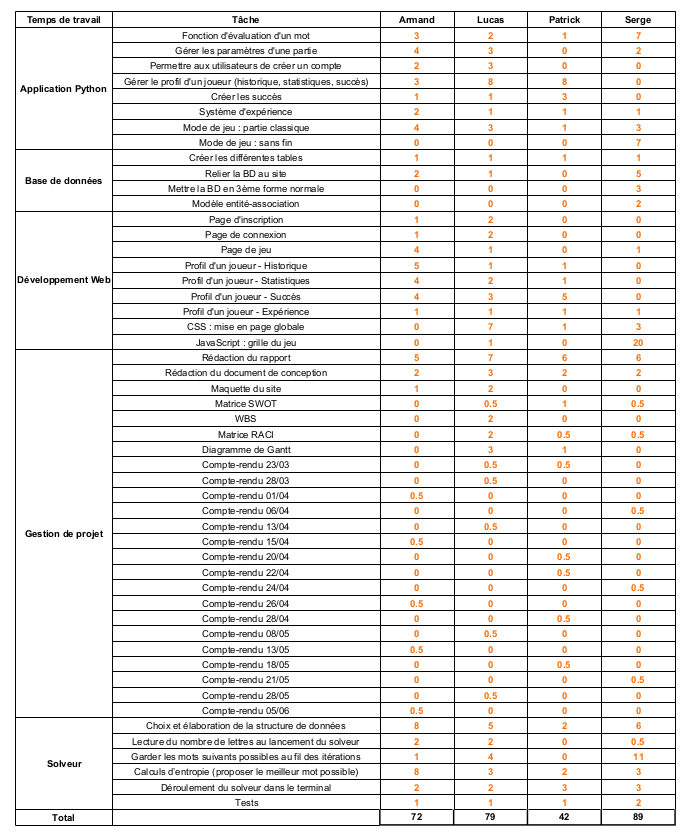
\includegraphics[width=16cm]{figures/Temps_travail.png}
    \caption{Volume horaire}
\end{figure}